% Clase del documento
\documentclass[12pt,twoside,titlepage]{report}





%%%%%%%%%%%%%%%%%%%%%%% Paquetes %%%%%%%%%%%%%%%%%%%%%%%

\usepackage[a4paper,bindingoffset=3mm,bottom=35mm]{geometry}


% Usad \usepackage[dvips]{graphicx} o \usepackage[pdftex]{graphicx} (no ambos)
%\usepackage[dvips]{graphicx} %%% para LaTeX. Las figuras deben estar en formato eps

\usepackage[colorlinks=true,pdftex]{hyperref}   %%% Opcional. Para incluir marcadores y enlaces en el pdf
\usepackage[pdftex]{graphicx}  %%% para pdflatex. Las figuras pueden estar en pdf, jpg, svg y otros formatos


\usepackage[spanish]{babel}

%\usepackage[latin1]{inputenc} % Usad en WinEdt/MikTex
\usepackage[utf8]{inputenc} % Usad en overleaf

%\usepackage[T1]{fontenc}


% Algunos paquetes útiles

\usepackage{amsmath,amssymb}
\usepackage{hyperref}
\usepackage{xcolor}
\usepackage{afterpage}
\usepackage{paralist}
\usepackage{array}
\usepackage{enumerate}
\usepackage{paralist}
\usepackage{enumitem}
\usepackage{float}
\usepackage{setspace}
\usepackage{listings}
\usepackage{algorithm}
\usepackage{algorithmic}
\usepackage{fancyhdr}
\usepackage{rotating}
\usepackage{multirow}


% Otros paquetes

\usepackage{quotchap}
\usepackage{lipsum}

%%%%%%%%%%%%%%%%%%%%%%%%%%%%%%%%%%%%%%%%%%%%%%%%%%%%%%%%






%%%%%%%%%%%%%%%%%%%%%%% Definiciones básicas %%%%%%%%%%%%%%%%%%%%%%%

\newcommand{\nombreautor}{Javier Raúl Alonso Tejera}
\newcommand{\nombretutor}{Michel Maes Bermejo}
\newcommand{\titulotrabajo}{OUTSIDER: UN JUEGO ONLINE EN TIEMPO REAL}
\newcommand{\escuela}{Escuela Técnica Superior\\de Ingeniería Informática}
\newcommand{\escuelalargo}{Escuela Técnica Superior de Ingeniería Informática}
\newcommand{\universidad}{Universidad Rey Juan Carlos}
\newcommand{\fecha}{Fecha}
\newcommand{\grado}{Grado en Ingeniería de Computadores}
\newcommand{\curso}{Curso 2023-2024}
\newcommand{\logoUniversidad}{logoURJC.pdf} % logoURJC.eps

%%%%%%%%%%%%%%%%%%%%%%%%%%%%%%%%%%%%%%%%%%%%%%%%%%%%%%%%%%%%%%%%%%%%






%%%%%%%%%%%%%%%%%%%%%%%%% Otras definiciones %%%%%%%%%%%%%%%%%%%%%%%%%%

% Definiciones de colores (para hidelinks)
\definecolor{BlueLink}{rgb}{0.165,0.322,0.745}
\definecolor{PinkLink}{rgb}{0.8,0.22,0.5}
\definecolor{gray}{rgb}{0.6,0.6,0.6}


% Enlaces
\hypersetup{hidelinks,pageanchor=true,colorlinks,citecolor=PinkLink,urlcolor=black,linkcolor=BlueLink}


\newcommand\blankpage{%
    \newpage
    \null
    \thispagestyle{empty}%
    %\addtocounter{page}{-1}%
    \newpage}


% Texto referencias
\addto{\captionsspanish}{\renewcommand{\bibname}{Bibliografía}}

% Texto Índice de tablas
\addto\captionsspanish{
\def\tablename{Tabla}
\def\listtablename{\'{I}ndice de tablas}
}


\floatname{algorithm}{Algoritmo}

\newfloat{algorithm}{t}{lop}

%% Etiquetas de comentarios (tutor/alumno)
\newif\ifdraft
\drafttrue
\usepackage{subcaption}
\newcommand{\nb}[2]{
	{
		{\color{black}{
				\small\fbox{\bfseries\sffamily\scriptsize#1}
				{\sffamily\small$\triangleright~${\it\sffamily\small #2}$~\triangleleft$}
	}}}
}

\ifdraft
\newcommand\tutor[1]{\nb{Tutor}{\color{red}#1}}
\newcommand\alumno[1]{\nb{Alumno}{\color{blue}#1}}
\newcommand\cotutor[1]{\nb{Co-tutor}{\color{green}#1}}
\newcommand{\fixme}[1]{{\textcolor{red}{[FIXME] #1}}\xspace}
\newcommand{\cn}{{\color{violet}[citation required]}}

\else
%\usepackage[disable]{todonotes}
\newcommand\tutor[1]{}
\newcommand\alumno[1]{}
\newcommand\cotutor[1]{}
\newcommand{\fixme}[1]{}
\newcommand{\cn}{}

\fi






%\newenvironment{pseudocodigo}[1][htb]
%  {\renewcommand{\algorithmcfname}{Pseudocódig}% Update algorithm name
%   \begin{algorithm}[#1]%
%  }{\end{algorithm}}
  
%%%%%%%%%%%%%%%%%%%%%%%%%%%%%%%%%%%%%%%%%%%%%%%%%%%%%%%%%%%%%%%%%%%%





%%%%%%%%%%%%%%%%%%%%%%% Estilo de código (en Python) %%%%%%%%%%%%%%%%%%%%%%%

\definecolor{bg}{rgb}{0.95,0.95,0.95}
\definecolor{mydeepteal}{rgb}{0.16,0.22,0.23}
\definecolor{myteal}{rgb}{0.31,0.44,0.46}
\definecolor{mymediumteal}{rgb}{0.41,0.58,0.60}

\DeclareFixedFont{\ttb}{T1}{txtt}{bx}{n}{12} % for bold
\DeclareFixedFont{\ttm}{T1}{txtt}{m}{n}{12}  % for normal


%\newcommand*{\FormatDigit}[1]{\textcolor{mydeepteal}{#1}}
\newcommand*{\FormatDigit}[1]{\textcolor{black}{#1}}

% Python style for highlighting
\newcommand\mypythonstyle{\lstset{
language=Python,
basicstyle=\ttfamily\small,
%basicstyle=\linespread{1.0}\footnotesize\ttm,
otherkeywords={self},             % Add keywords here
keywordstyle=\bfseries\ttfamily\color{myteal},
%keywordstyle=\ttb\color{myteal},
commentstyle=\itshape\color{myteal},
stringstyle=\color{mydeepteal},
emph={MyClass,__init__},          % Custom highlighting
emphstyle=\ttb\color{mydeepteal},    % Custom highlighting style
% Any extra options here
showstringspaces=false,            %
backgroundcolor=\color{bg},
rulecolor = \color{bg},
%identifierstyle=\color{deepgreen},
breaklines=true,
numbers=left,
numbersep=5pt,
numberstyle=\tiny,
tabsize=4,
xleftmargin=1em,
frame = single,
framesep = 3pt,
framextopmargin=0pt,
framexbottommargin=0pt,
framexleftmargin=0pt,
framexrightmargin=0pt,
fontadjust=true,
basewidth=0.55em, % compactness of code
upquote=true,
}}

% Python environment
\lstnewenvironment{mypython}[1][]
{
\mypythonstyle
\lstset{#1}
}
{}

\newcommand\mypythonstylenormalinline{\lstset{
language=Python,
basicstyle=\ttfamily\normalsize,
%basicstyle=\linespread{1.0}\footnotesize\ttm,
otherkeywords={self},            % Add keywords here
keywordstyle=\bfseries\ttfamily\color{myteal},
%keywordstyle=\ttb\color{myteal},
commentstyle=\itshape\color{mymediumteal},
stringstyle=\color{mydeepteal},
emph={MyClass,__init__},          % Custom highlighting
emphstyle=\ttb\color{mydeepteal},    % Custom highlighting style
% Any extra options here
showstringspaces=false,            %
backgroundcolor=\color{bg},
rulecolor = \color{bg},
%identifierstyle=\color{deepgreen},
breaklines=false,
numbers=left,
numbersep=5pt,
numberstyle=\tiny,
tabsize=4,
xleftmargin=0em,
frame = single,
framesep = 3pt,
framextopmargin=0pt,
framexbottommargin=0pt,
framexleftmargin=0pt,
framexrightmargin=0pt,
fontadjust=true,
%basewidth=0.55em, % compactness of code
upquote=true,
}}

\newcommand\mypythoninline[1]{{\mypythonstylenormalinline\lstinline!#1!}}

%%%%%%%%%%%%%%%%%%%%%%%%%%%%%%%%%%%%%%%%%%%%%%%%%%%%%%%%%%%%%%%%%%%%%%%%%%%%%%




%%%%%%%%%%%%%%%%%%%%%%%%%%%% Comandos definidos por el autor 

\newcommand{\transpuesta}{\mbox{\tiny $\mathsf{T}$}}








%%%%%%%%%%%%%%%%%%%%%%%%%%%%%%%%%%%%%%%%%%%%%%%%%%%%%%%%%%%%%%%%%%%%%%%
%                           Inicio del documento                       
%%%%%%%%%%%%%%%%%%%%%%%%%%%%%%%%%%%%%%%%%%%%%%%%%%%%%%%%%%%%%%%%%%%%%%%


\begin{document}

\pagestyle{plain}




%%%%%%%%%%%%%%%%%%%%%%%%%%%%%%%%%%%% Portada %%%%%%%%%%%%%%%%%%%%%%%%%%%%%%%%%%

%\pagenumbering{gobble}
%\pagenumbering{arabic}

% Universidad, Facultad
\begin{titlepage}
	\selectlanguage{spanish}
						
						
	% logo
	\begin{center}
		\includegraphics[scale=0.7]{\logoUniversidad}
	\end{center}
						
	\bigskip
						
	\begin{center}
		\begin{LARGE}
			\escuela \\
		\end{LARGE}
	\end{center}
						
	\bigskip
	\bigskip
						
	% Grado
	\begin{center}
		\begin{large}
			\textbf{\grado}\\
		\end{large}
	\end{center}
						
	% Curso
	\begin{center}
		\begin{large}
			\textbf{\curso}\\
		\end{large}
	\end{center}
						
	\bigskip
						
	\textbf{\begin{center}
		\begin{large}
			\textbf{Trabajo Fin de Grado}
		\end{large}
		\end{center}}
						
	\bigskip
	\bigskip
	\bigskip
						
	% Nombre del TFG
	\begin{center}
		\textbf{\begin{large}
			\MakeUppercase{\titulotrabajo}\\
			\end{large}}
	\end{center}
						
	% Nombre del autor
	\vspace{\fill}
	\begin{center}
		\textbf{Autor: \nombreautor}\\ \smallskip
		% Tutor
		\textbf{Tutor: \nombretutor}\\
		% Añadir segundo tutor si hubiera
												
												
		\bigskip
												
		% Fecha
		%\textbf{\fecha}\\
	\end{center}
\end{titlepage}


%%%%%%%%%%%%%%%%%%%%%%%% Opcional %%%%%%%%%%%%%%%%%%%%%%
%\blankpage

%\thispagestyle{empty}
%\begin{center}

% Nombre del trabajo
%\textbf{\begin{large}
%\MakeUppercase{\titulotrabajo}\\*
%\end{large}}
%\vspace*{0.2cm}
%\vspace{5cm}

% Nombre del autor y del tutor
%\large Autor: \nombreautor \\* \medskip
%\large Tutor: \nombretutor \\*

%\vfill

% Escuela, universidad y fecha
%\escuelalargo \\ \smallskip
%\universidad \\
%\vspace{1cm}
%\fecha \\

%\clearpage

%\end{center}
%%%%%%%%%%%%%%%%%%%%%%%%%%%%%%%%%%%%%%%%%%%%%%%%%%%%%%%%

\hypersetup{pageanchor=true}

\normalsize
\afterpage{\blankpage} % Se deben añadir página en blanco para que lo capítulos de la memoria o estas secciones introductorias empiecen en páginas impares

%%%%%%%%%%%%%%%%%%%%%%%%%%%%%%%%%%%%%%%%%%%%%%%%%%%%%%%%%%%%%%%%%%%%%%%%%%%%%%%





% Estilo de párrafo de los capítulos
\setlength{\parskip}{0.75em}
\renewcommand{\baselinestretch}{1.25}
% Interlineado simple
\spacing{1}

\pagenumbering{Roman}
\setcounter{page}{2}


%%%%%%%%%%%%%%%%%%%%%%%%% Agradecimientos o dedicatoria %%%%%%%%%%%%%%%%%%%%%%%%%%%

\chapter*{Agradecimientos}

Breves agradecimientos o dedicatoria.

\afterpage{\blankpage}

%%%%%%%%%%%%%%%%%%%%%%%%%%%%%%%%%%%%%%%%%%%%%%%%%%%%%%%%%%%%%%%%%%%%%%%%%%%%%%%%%%%






%%%%%%%%%%%%%%%%%%%%%%%%%%%%%%%%%%%% Resumen %%%%%%%%%%%%%%%%%%%%%%%%%%%%%%%%%%%%%%

\chapter*{Resumen}

Breve resumen del Trabajo de Fin de Grado (TFG). Recomendable entre 250-300 palabras, conteniendo los principales objetivos y resultados derivados del mismo.

\mbox{} \bigskip

\noindent \textbf{Palabras clave}:
\begin{compactitem}
	\item Python
	\item Ciberseguridad
	\item Aprendizaje automático (pueden ser varias)
	\item $\ldots$
\end{compactitem}

\afterpage{\blankpage}

%%%%%%%%%%%%%%%%%%%%%%%%%%%%%%%%%%%%%%%%%%%%%%%%%%%%%%%%%%%%%%%%%%%%%%%%%%%%%%%%%%%





%%%%%%%%%%%%%%%%%%%%%%%%%%%%%%%%%%%% Índices %%%%%%%%%%%%%%%%%%%%%%%%%%%%%%%%%%%%

% Estilo de párrafo de los Índices
\setlength{\parskip}{1pt}
\renewcommand{\baselinestretch}{1}
\renewcommand{\contentsname}{Índice de contenidos}


% Índice de contenidos
\tableofcontents
\afterpage{\blankpage}

% Índice de tablas (OPCIONAL)
\listoftables
\afterpage{\blankpage}
\addcontentsline{toc}{chapter}{\noindent \listtablename}

% Índice de figuras (OPCIONAL)
\listoffigures
\afterpage{\blankpage}
\addcontentsline{toc}{chapter}{\listfigurename}

% Índice de códigos/algoritmos (OPCIONAL).   El término "Códigos" se puede cambiar por "Métodos", "Funciones", "Algoritmos", etc.
\renewcommand\lstlistlistingname{Códigos}
\renewcommand\lstlistingname{Código}
\renewcommand\lstlistlistingname{Índice de códigos}

\lstlistoflistings
\afterpage{\blankpage}
\addcontentsline{toc}{chapter}{\lstlistlistingname}


% En este documento (de momento) no se ha considerado incluir un índice de algoritmos/pseudocódigos, como el que aparece en \ref{AdditionalLouvain}

%%%%%%%%%%%%%%%%%%%%%%%%%%%%%%%%%%%%%%%%%%%%%%%%%%%%%%%%%%%%%%%%%%%%%%%%%%%%%%%%%%%





%%%%%%%%%%%%%%%%%%%%%%% Cabeceras y pies de página (Opcional) %%%%%%%%%%%%%%%%%%%%%%%

%\setlength{\headheight}{15.2pt}
\pagestyle{fancy}


\renewcommand{\chaptermark}[1]{\markboth{Capítulo \thechapter.\ #1}{}}

\pagestyle{fancy}
\fancyhf{}
\fancyhead[LO]{\leftmark}
\fancyhead[RO]{}
\fancyhead[RE]{\nouppercase\rightmark}
\fancyhead[LE]{}
\fancyfoot[C]{\thepage}

%%%%%%%%%%%%%%%%%%%%%%%%%%%%%%%%%%%%%%%%%%%%%%%%%%%%%%%%%%%%%%%%%%%%%%%%%%%%%%%%%%%%






%%%%%%%%%%%%%%%%%%%%%%%%%%%%%% Capítulos de la memoria %%%%%%%%%%%%%%%%%%%%%%%%%%%%%



% Capítulo 1
\chapter{Introducción}


%%%%%%%%%%%%%%%%%%%%%%%%%%%%%%%%%%%%%%%%%%%%%%%%%%%%%%%%%%%%%%%%%%%%%%%%%%

% Estilo resto de páginas
\pagestyle{fancy}


% Estilo de párrafo de los capítulos
\setlength{\parskip}{0.75em}
\renewcommand{\baselinestretch}{1.25}
% Interlineado simple
\spacing{1}
% Numeración contenido
\pagenumbering{arabic}
\setcounter{page}{1}

%%%%%%%%%%%%%%%%%%%%%%%%%%%%%%%%%%%%%%%%%%%%%%%%%%%%%%%%%%%%%%%%%%%%%%%%%%

Este documento aborda y explica el desarrollo de este proyecto de fin de grado,
desde su concepción inicial y las motivaciones que lo impulsaron, hasta los detalles
finales de su implementación.

\section{Descripción general}

El objetivo general del proyecto es el desarrollo de un juego multijugador web de adivinanza de palabras y roles ocultos. El principal punto de interés
radica en el uso de tecnologías en tiempo real, específicamente de tecnologías websocket, posibilitando el juego online entre los jugadores
de forma fiable y óptima.

Las mecánicas base del juego son sencillas y son más una adaptación de un tipo de juego que normalmente se realiza sin el uso de tecnologías informáticas.
El concepto más básico del juego se podría resumir mediante los siguientes puntos:

\begin{enumerate}
	\item En este juego, todos los jugadores juegan como ``Inocentes'', a excepción de uno de ellos,
	      definido como el ``Outsider''.
	\item Al empezar la partida, los jugadores
	      Inocentes reciben una
	      palabra secreta o contraseña, como por ejemplo, ``Hoja''.
	\item  Siguiendo un orden secuencial (con el primer jugador elegido al azar), cada
	      participante debe escribir una palabra relacionada con su palabra clave
	      para indicar a los demás que conocen la palabra asignada.
	\item Por ejemplo si la palabra clave es la palabra ``Hoja'', unas palabras que
	      alienten a esta  o palabra clave podrían ser ``Árbol'', ``Libro'' o ``Afeitado''.
	\item El jugador designado como Outsider, quien no tiene conocimiento de la palabra secreta, debe tratar de deducirla a partir de las palabras
	      previamente mencionadas y decir una palabra que no levante sospechas.
	\item Después de que todos los jugadores hayan compartido una palabra, se lleva a cabo una votación simultánea, donde cada jugador vota por la persona que creen
	      que es el Outsider.
	\item El Outsider ganará si no es el jugador más votado. Por otra parte, el resto de los jugadores Inocentes ganarán
	      si logran descubrir al Outsider y este llega a ser el jugador más votado.
\end{enumerate}

Dadas estas reglas de funcionamiento del juego, el desarrollo del proyecto consiste principalmente en
interpretar y diseñar una aplicación web capaz de poder gestionar todos estos puntos. En el próximo capítulo de Objetivos (\ref{Objetivos}),
se tratará con más detalle esta definición de reglas.

Además de generar una aplicación/juego que emule estas reglas, es bastante destacable el trabajo adicional relacionado con la gestión informática que
implica desarrollar una aplicación web: desde el diseño de interfaces usables hasta su despliegue y testeo, todos estos apartados se trataran en detalle
como parte del desarrollo.

\section{Motivación}

La principal motivación para la realización de este proyecto es el aprendizaje propio. La idea del juego
surge por parte del tutor del TFG, \nombretutor, que ve muy interesante la creación de una aplicación que haga uso de tecnologías en
tiempo real. También ha sido una figura clave en el desarrollo iterativo del proyecto, proponiendo mejoras y comentarios
a las diferentes versiones de la aplicación.

Dicho esto, a día de hoy hay innumerables proyectos, aplicaciones y juegos que persiguen conseguir un rendimiento económico o lúdico, sin embargo, también es importante destacar el papel
de la investigación y el aprendizaje, especialmente en el ámbito académico en el que se sitúa este trabajo de fin grado.

Las empresas y organizaciones buscan desarrolladores software altamente capacitados, pero también especializados en materias en concreto.
Destaca más un desarrollador que sepa sobre una tecnología útil y difícil de aprender sobre otro que sepa
sobre otra tecnología menos útil o mucho más accesible. Aquí es donde entran en juego los websockets, cuyas implementaciones suelen dar problemas 
a los desarrolladores.

Muchos estudiantes hemos realizado pequeños proyectos y pruebas con websockets y tecnologías análogas, pero es muy diferente desarrollar toda una aplicación, realizar testing e
incluso llevar a cabo un despliegue en torno a tecnologías en tiempo real. Hay que tener en cuenta muchas variables y por otra parte se tratan de tecnologías útiles
con infinidad de aplicaciones. Desde un simple chat en línea al uso de websockets en grandes proyectos, el uso de aplicaciones web en tiempo real es muy práctico.

Desde mi experiencia previa en desarrollo de aplicaciones móviles, un desarrollador no es consciente de la cantidad de lógica que se necesita para manejar una base
de datos en lo que a priori se presenta como una sencilla aplicación. Todo el trabajo subyacente es muy poco conocido pero suele ser de gran importancia. En este trabajo previo,
se destaca que se planteó varias veces la necesidad de poder crear conexiones websockets entre usuarios de la aplicación para poder compartir datos de forma inmediata.

Las aplicaciones que usamos en nuestros teléfonos y dispositivos, los videojuegos online o los servicios de streaming 
dependen de una estructura muy bien pensada para cada caso específico. Por ello, es una necesidad por parte de un desarrollador software, 
al menos entender, como funcionan todos estos sistemas. Mi objetivo es explorar y aprender lo máximo de la mayor cantidad de tecnologías 
software para desarrollarme como profesional así como para enseñar las posibilidades que ofrecen estas diversas herramientas.


% \afterpage{\blankpage} % puede generar problema en índice de contenidos
% \newpage


% Capítulo 2
\chapter{Objetivos}

En esta sección se definirán los objetivos principales del proyecto así como de otros objetivos y
requisitos secundarios que han ido definiéndose a lo largo del proyecto.

\section{Objetivos funcionales del juego} \label{Objetivos}

En primera instancia destacamos las funcionalidades básicas que debería cumplir el juego como
producto software, es decir, relacionados con el usuario de forma directa.

\subsection{Funcionalidad básica, lobby y conexiones}

Además del propio juego, es necesario dar las capacidades y herramientas necesarias a los usuarios para
poder organizar partidas de forma sencilla. Para ello se plantea la creación de una página de inicio que
permita al usuario poder crear salas de juego o unirse a salas ya creadas.

El objetivo en detalle sería permitir a todos los usuarios de la aplicación poder jugar a
diferentes partidas, teniendo en cuenta varias limitaciones como el que un jugador no debería poder acceder
a una partida ya empezada o evitar la creación de salas con el mismo nombre. De forma adicional, en esta página se deberían mostrar instrucciones que expliquen el funcionamiento
del juego.

También sería esencial tener una pantalla pre-partida en la cual se vayan uniendo los jugadores
antes de comenzar el juego. En esta pantalla se propone añadir un chat para los jugadores además
de mostrar la información pertinente al estado de la partida: número de jugadores preparados, código de la
sala para que se puedan unir más jugadores, etc.

\subsection{Juego sencillo}

En primer lugar, se plantea poder jugar de forma sencilla solo una ronda en la cual se deciden los
roles de los jugadores y se les indica una palabra clave a los jugadores Inocentes. Esta palabra 
clave es desconocida por el Outsider y el resto de jugadores Inocentes deberán demostrar 
que la conocen mientras evitan desvelarla al verdadero jugador Outsider. Se destaca 
que ninguno de los jugadores debería conocer a ciencia cierta el rol de otro, por ello, se trata de un juego 
con un alto factor de interacción social, donde la intuición y la discreción son elementos clave.

Con la palabra clave revelada a los jugadores Inocentes, se procede con la lógica de juego estándar: cada jugador siguiendo 
un orden secuencial, escribirá una palabra relacionada con su palabra clave
para indicar a los demás que conocen la palabra asignada; después de que todos los jugadores hayan compartido una
palabra, se lleva a cabo una votación simultánea, donde cada jugador vota por la persona que creen
que es el Outsider.

El Outsider ganará si no es el jugador más votado. Por otra parte, el resto de los jugadores Inocentes ganarán
si logran descubrir al Outsider y este llega a ser el jugador más votado.

El objetivo es llevar a cabo la implementación de esta lógica de la forma más consistente posible, trabajando en
detalle las conexiones websocket.

\subsection{Última oportunidad}

Habiendo implementado el juego sencillo, se quiere añadir nuevas funcionalidades base. En primer lugar, dado el transcurso
normal del juego, tras la votación simultánea, en el caso de que el Outsider reciba la mayoría de los votos, se le otorgará
una última oportunidad para ganar adivinando la palabra clave.

\subsection{Múltiples rondas}

Cuando existen más de tres jugadores en una partida, se detecta la necesidad de poder jugar varias rondas,
ya que, si no se elimina al Outsider inicialmente y se elimina a un jugador Inocente, podrían seguir jugando el resto de jugadores
rondas adicionales.

Los jugadores eliminados pasan a ser espectadores mientras el resto sigue jugando hasta que no 
se pueda seguir el juego porque solo queden un jugador Outsider y otro Inocente (en este caso
ganaría el Outsider de forma definitiva) o se elimine mediante votación al Outsider en cuestión.

\subsection{Varios Outsider}

Relacionado con el anterior punto, en partidas con varios jugadores se ve necesario aumentar el número de Outsiders en aras de
una jugabilidad más interesante. De esta manera, se plantea que cuando el número de jugadores sea mayor que seis, simplemente sean
dos jugadores Outsider en la partida.

En estos casos el Outsider solo tendrá la oportunidad de adivinar la palabra clave si es el último Outsider en la partida. Por contraparte, si 
todavía hay dos Outsiders jugando y solo quedan otros dos jugadores Inocentes sin eliminar, ganaría el bando Outsider al tener ventaja en los 
votos.

\section{Objetivos secundarios y tecnológicos}

Dados los objetivos/reglas principales que debería cumplir el juego, se añaden varios puntos adicionales que se quieren
tratar como objetivos secundarios del proyecto.

\subsection{Plataforma de juego}

Se quiere aprovechar el uso de un entorno web para hacer más accesible el juego a diferente tipo de usuarios.

El objetivo es hacer usable la aplicación en el mayor número de dispositivos posibles diferenciando principalmente entre
teléfonos móviles y equipos de escritorio (ordenadores y portátiles esencialmente). Se diferencia entre estos dos tipos de
dispositivos porque también se prevén dos tipos de juego de forma predominante:

\begin{compactitem}
    \item Juego presencial en un mismo espacio físico.
    \item Juego remoto.
\end{compactitem}

Se entiende que si un grupo quiere jugar en un espacio físico común, por ejemplo, en un cumpleaños en la casa de uno de los
jugadores, en la mayoría de casos todos los jugadores jugarán con sus propios dispositivos móviles, principalmente smartphones.

Por otro lado, también se ve bastante común que otro grupo de jugadores quiera jugar de forma remota, cada uno en una
localización diferente. En este caso, se podría asumir que la mayoría de jugadores intentarían jugar con sus dispositivos de
escritorio.

\subsection{Testing}

Se propone de forma adicional trabajar ciertos elementos de Integración Continua (CI, por sus siglas en inglés), especialmente el testing del software, ya que, es una práctica
esencial en la industria y resulta bastante llamativo trabajar el testing con tecnologías en tiempo real.

\subsection{Despliegue}

Para poder enseñar el resultado del proyecto de la forma más accesible posible, también se quiere trabajar con tecnologías de
AWS (Amazon Web Services) para poder tener la aplicación desplegada y totalmente disponible para cualquier usuario a la hora
de acceder a esta.

De esta forma se pretende aprender sobre tecnologías de despliegue y de crear una mejor presentación final del proyecto.

\subsection{Feedback de usuarios}

Para finalizar con la descripción inicial de objetivos, se pretende realizar una pequeña prueba con usuarios a mitad de
desarrollo con el objetivo de encontrar bugs y pequeñas mejoras para el juego, lo que generará su propia lista de cambios a realizar.

\section{Resumen de objetivos}

\begin{enumerate}
    \item Gestionar las conexiones entre jugadores mediante salas.
    \item Creación del juego básico.
    \item Añadir una mecánica adicional a la hora de eliminar al último jugador Outsider.
    \item Permitir jugar varias rondas.
    \item Añadir más jugadores Outsider al juego si hay muchos jugadores en partida.
    \item Gestionar la usabilidad de la aplicación en diferentes dispositivos.
    \item Tener en cuenta el feedback de los usuarios. Testing manual.
    \item Realización de tests para la lógica en tiempo real. Testing automático.
    \item Desplegar la aplicación a través de tecnologías modernas.
\end{enumerate}

\blankpage

% Capítulo 3
\chapter{Contenidos principales}
\label{chap:contenidos}

\section{Primera sección}

% Citar una referencia
Esto es una referencia bibliográfica \cite{bibex}. Se recomienda leer ``The Not So Short Introduction to \LaTeX'' \cite{Oetiker2007} (existen versiones más modernas).


\subsection{Ecuaciones y fórmulas}

Gracias a la ecuación de Euler ($e^{ \pm i\theta } = \cos \theta \pm i\sin \theta$) podemos ver la relación entre varias de las constantes matemáticas más importantes:
\[
    e^{i\pi} + 1 = 0.
\]


% Fórmula numerada
Si una ecuación se va a referenciar es necesario numerarla:
\begin{eqnarray}
\label{eq:schemeP}
 \Phi (k)=\dfrac{2}{|R(k)|(|R(k)|-1)} \underset{i,j \in R(k)}{\sum} a_{ij}.
\end{eqnarray}
Posteriormente se hace referencia a la ecuación a través de su etiqueta (label). Por ejemplo, la anterior ecuación \eqref{eq:schemeP}.



Problema de optimización:
\begin{equation}\label{eq:LP1}
\begin{array}{cl}
  \displaystyle \begin{array}{c}\mathrm{minimizar} \\ \mathbf{t} \in \mathbb{R}^{n}, \  \mathbf{p} \in \mathbb{R}^{m} \end{array} & \hspace{-0.2cm} \begin{array}{c} \mathbf{1}^{\transpuesta}\mathbf{t} \\ \mbox{} \end{array}  \\
  & \vspace{-0.4cm} \\ % línea (fila) en blanco, pero la hacemos estrecha con el comando vspace
  \mbox{sujeto a} & -\mathbf{t} \preceq  \mathbf{V}\mathbf{p} - \mathbf{x}  \preceq  \mathbf{t},\\
 \end{array}
\end{equation}




\subsection{Tablas y figuras}

% Insertar una tabla
\begin{table}
  \centering
  \caption{Título de la tabla.}
  \label{tab:una_tabla}

\begin{footnotesize}
\renewcommand{\arraystretch}{1.5} % Para cambiar la separación entre filas (1 por defecto)
\begin{tabular}{ccccccccccc}
  \hline
   & Subs. & Students & A & PE & WA & RE & CTE & IF & TLE & All\\
  \hline
Ex. 1 & 104 & 44 & 1.27    &   0       &   0.55    &   0.23    &   0.20    &   0.11    &   0     & 2.36  \\
Ex. 2 & 118 & 37 & 0.92    &   0       &   0.92    &   0.27    &   0.49    &   0.59    &   0     & 3.19  \\
Ex. 3 & 100 & 28 & 1.21    &   0.39    &   1.18    &   0.54    &   0.14    &   0.07    &   0.04  & 3.57  \\
Ex. 4 & 78  & 25 & 1.08    &   0.84    &   0.52    &   0.40    &   0.24    &   0.04    &   0     & 3.12  \\
Ex. 5 & 116 & 31 & 1.48    &   0.10    &   0.77    &   0.32    &   0.42    &   0.19    &   0.45  & 3.74  \\
Ex. 6 & 213 & 32 & 1.06    &   0.34    &   3.81    &   0.56    &   0.69    &   0.06    &   0.13  & 6.66  \\
Ex. 7 & 116 & 34 & 1.35    &   0.38    &   0.38    &   0.68    &   0.62    &   0       &   0     & 3.41  \\
  \hline
Average & 120.7 & 33 & 1.20 &  0.26 &  1.14 &  0.42 &  0.40 &  0.16 &  0.08 & 3.66 \\
  \hline
 \end{tabular}
\end{footnotesize}

\end{table}









\begin{sidewaystable}
  \centering
  \caption{Tabla rotada. Factor groupings for the Mooshak questionnaire.}\label{tab:factor_analysis}

\renewcommand{\arraystretch}{1.1}
\begin{scriptsize}
 \begin{tabular}{clcc}
   \hline
   Factor & \textbf{Interpretation} / Items$^{*}$ (loadings)  & Median & Mode \\
   \hline
   \hline
    1 & \multicolumn{3}{l}{\textbf{Students' perception of Mooshak towards its helpfulness in learning} } \\
   \hline
    (21.17\%) & m10. Mooshak has forced me to implement programs more carefully $(0.849)$ & 4 & 4 \\
    $\alpha$ = 0.922 & m6.  Mooshak has helped me improve as a programmer $(0.819)$ & 3 & 4 \\
     & m5.  Mooshak has made me more aware of the need to write correct code $(0.781)$ & 3 & 3\\
     & m1. Mooshak has forced me to program more responsibly $(0.713)$ & 3 & 3 \\
     & m15. The specifications regarding the exercises used with Mooshak are adequate $(0.687)$ & 3 & 3 \\
     & m18. Mooshak helps to measure my current programming skills $(0.680)$ & 2.5 & 3 \\
   \hline
%   \multicolumn{4}{c}{} \vspace{-0.2cm}\\
%   \hline
    2 & \multicolumn{3}{l}{\textbf{Disposition towards using Mooshak} } \\
   \hline
    (17.93\%) & m24. I would be willing to participate in a programming contest using Mooshak, with similar exercises to the ones & 2 & 1 \\
    $\alpha$ = 0.897 & seen throughout the course $(0.807)$ & & \\
    & m13. Using Moohak in the final exams is a good idea $(0.748)$ & 2 & 1 \\
    & m14. I would like to use Mooshak or a similar tool in the future $(0.734)$ & 3 & 1 \\
    & m17. Knowing Mooshak can motivate me to take part in a programming contest $(0.655)$ & 2 & 1\\
    & m9. It would have been useful to use Mooshak from the first programming course $(0.527)$ & 2.5 & 1\\
     & m16. Using Mooshak in the course has been interesting $(0.522)$ & 3 & 4 \\
   \hline
%   \multicolumn{4}{c}{} \vspace{-0.2cm}\\
%   \hline
    3 & \multicolumn{3}{l}{\textbf{Effect of Mooshak's feedback in the tool's usefulness} } \\
   \hline
    (14.84\%) & m12. Mooshak's feedback is adequate $(0.832)$ & 2 & 1\\
    $\alpha$ = 0.836 & m3. Using Mooshak has increased my workload considerably $(0.693)$ & 4 & 4 \\
     & m7.  If Mooshak does not accept my code I feel motivated to find and fix the errors $(0.691)$ & 2 & 3 \\
     & m8.  In general, using Mooshak has been a good idea $(0.666)$ & 3 & 4 \\
   \hline
%   \multicolumn{4}{c}{} \vspace{-0.2cm}\\
%   \hline
    4 & \multicolumn{3}{l}{\textbf{Mooshak's effect on persistence} } \\
   \hline
    (11.20\%) & m23. When Mooshak does not accept my code I get discouraged and I abandon the exercise $(0.848)$ & 3 & 3 \\
    $\alpha$ = 0.705 & m22. Mooshak has been a waste of time $(0.597)$ & 2 & 2 \\
    & m25. Once a program has passed Mooshak's tests, I rewrite it in order to enhance it $(0.559)$ & 2 & 2 \\
   \hline
%   \multicolumn{4}{c}{} \vspace{-0.2cm}\\
%   \hline
   5 & \multicolumn{3}{l}{\textbf{Students' perception of Mooshak's features} } \\
   \hline
    (10.87\%) & m20. Even if it is not related to the grade, I feel satisfied if I am one of the first students to complete an exercise $(0.729)$ & 2 & 2\\
   $\alpha$ = 0.742  & m19. I value the fact that a tool like Mooshak returns feedback in real time about the correction of my programs $(0.650)$ & 3.5 & 4 \\
   \hline
%   \multicolumn{4}{c}{} \vspace{-0.2cm}\\
%   \hline
\multicolumn{4}{l}{\scriptsize $^{*}$Measured on a 5-point Likert scale (1: strongly disagree; 2: disagree; 3: neutral; 4: agree; 5: strongly agree).}
  \end{tabular}
\end{scriptsize}
\end{sidewaystable}



\begin{table}
  \centering

\begin{small}
\begin{tabular}{|l|l|l|l|}\hline
  \multirow{10}{*}{numeric literals} & \multirow{5}{*}{integers} & in decimal & \verb|8743| \\ \cline{3-4}
  & & \multirow{2}{*}{in octal} & \verb|0o7464| \\ \cline{4-4}
  & & & \verb|0O103| \\ \cline{3-4}
  & & \multirow{2}{*}{in hexadecimal} & \verb|0x5A0FF| \\ \cline{4-4}
  & & & \verb|0xE0F2| \\ \cline{2-4}
  & \multirow{5}{*}{fractionals} & \multirow{5}{*}{in decimal} & \verb|140.58| \\ \cline{4-4}
  & & & \verb|8.04e7| \\ \cline{4-4}
  & & & \verb|0.347E+12| \\ \cline{4-4}
  & & & \verb|5.47E-12| \\ \cline{4-4}
  & & & \verb|47e22| \\ \cline{1-4}
  \multicolumn{3}{|l|}{\multirow{3}{*}{char literals}} & \verb|'H'| \\ \cline{4-4}
  \multicolumn{3}{|l|}{} & \verb|'\n'| \\ \cline{4-4}          %% here
  \multicolumn{3}{|l|}{} & \verb|'\x65'| \\ \cline{1-4}        %% here
  \multicolumn{3}{|l|}{\multirow{2}{*}{string literals}} & \verb|"bom dia"| \\ \cline{4-4}
  \multicolumn{3}{|l|}{} & \verb|"ouro preto\nmg"| \\ \cline{1-4}          %% here
\end{tabular}
\end{small}

  \caption{Tabla con ``multicolumnas'' y ``multifilas''.}\label{tab:tablacompleja}
\end{table}





% Insertar una figura
\begin{figure}
  \centering
  \includegraphics[width=0.75\textwidth,clip=true]{\logoUniversidad}
  \caption{Logo de la Universidad.}
  \label{fig:logo_universidad}
\end{figure}

% Referenciar una etiqueta (label)
Las tablas y figuras deben presentarse en el texto, referenciadas y numeradas. La descripción de una figura debe ir posicionada debajo de la misma. Las descripciones de tablas pueden aparecer encima o debajo de las mismas (pero de forma consistente en todo el documento).

En las tablas se recomienda evitar líneas verticales y usar pocas horizontales. 

La figura~\ref{fig:logo_universidad} se utiliza en la portada. \LaTeX ubica automáticamente las tablas y figuras. Para ello emplea reglas basadas en la experiencia de profesionales de la edición de textos. Podemos forzar su ubicación, pero en general es recomendable usar la ubicación sugerida por el sistema \LaTeX. Usad gráficos vectoriales siempre que podáis.





\begin{figure}
   \centering

  \begin{minipage}{0.45\textwidth}
   \centering

     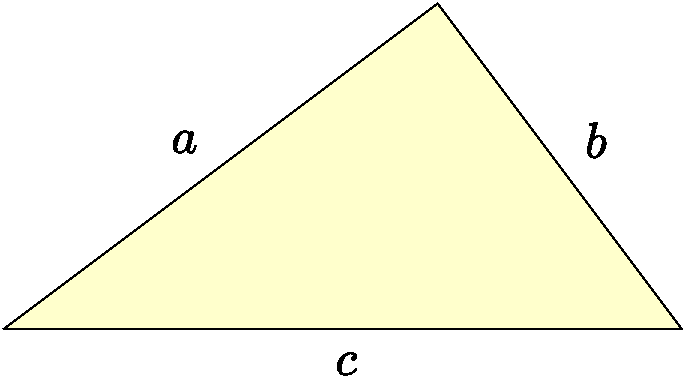
\includegraphics[clip=true,width=\textwidth]{triangulo_grande_bb.pdf}\\

    \footnotesize (a)
  \end{minipage}
  \hfill
  \begin{minipage}{0.45\textwidth}
   \centering
     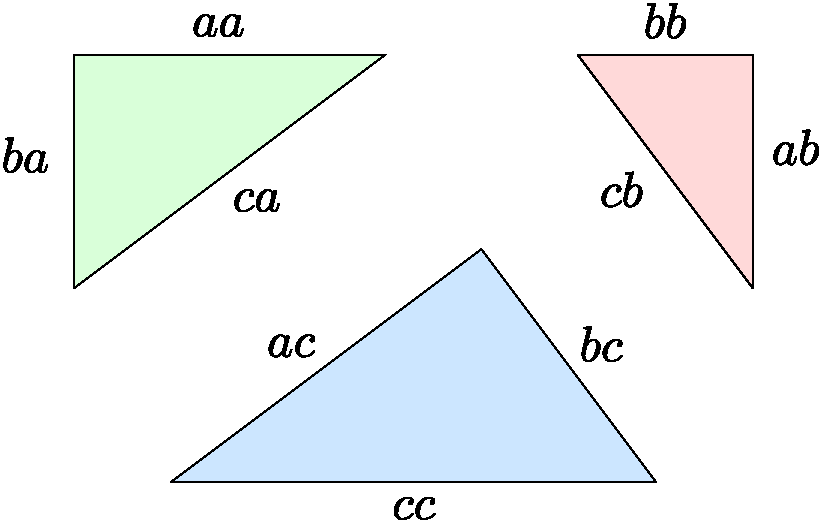
\includegraphics[clip=true,width=\textwidth]{triangulos_separados_bb.pdf}\\

   \footnotesize (b)
  \end{minipage}

    \bigskip

    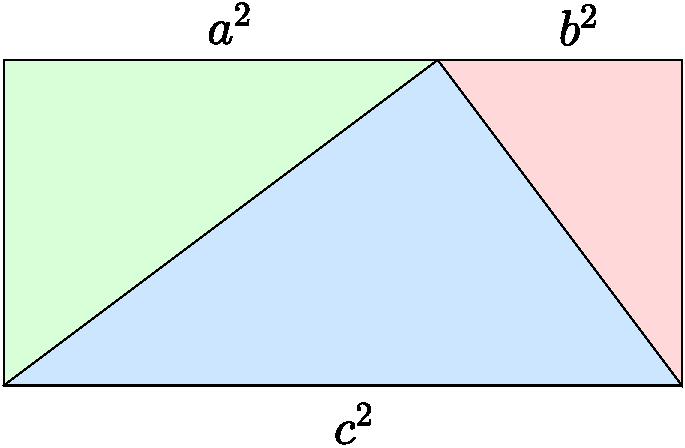
\includegraphics[clip=true,width=0.5\textwidth]{triangulos_unidos_bb.pdf}\\
    \footnotesize (c)

  \caption{Ejemplo con varias figuras. Demostración visual del teorema de Pitágoras. En (a) tenemos un triángulo rectángulo con hipotenusa $c$ y catetos $a$ y $b$. En (b) se muestra tres copias escaladas del mismo triángulo. El verde se ha escalado por $a$, el rojo/rosa por $b$, y el azul por $c$. En (c) se juntan los triángulos de (b) para formar un rectángulo cuya base es $c^{2}$, pero también $a^{2} + b^{2}$. Por tanto, $a^{2} + b^{2} = c^{2}$.}\label{fig:teoremapitagoras}
\end{figure}





\section{Segunda sección}

% Nueva página
Normalmente no tendremos que insertar saltos de página, salvo para forzar que los capítulos empiecen en páginas impares, con \begin{verbatim}\blankpage\end{verbatim} En cualquier caso, podemos introducir un salto de página con el comando \begin{verbatim}\newpage\end{verbatim}.

\newpage
% También con \pagebreak



\subsection{Código}


\begin{mypython}[float={!t},caption={Titulo del algoritmo/código.},label={alg:etiqueta}]
def sum_list_limits_1(a, lower, upper):
    if lower > upper:
        return 0
    else:
        return a[upper] + sum_list_limits_1(a, lower, upper - 1)
\end{mypython}
El código~\ref{alg:etiqueta} es un ejemplo en Python.



\begin{algorithm}
\begin{algorithmic}[1]
\STATE $\forall i \in V$, \ let $i$ be an isolated community
\STATE $o=permutation(V)$
\FOR{$k \ \in \ o$}
\STATE search in $A$ all the neighbours of $k$, $j$
\STATE $\forall j$, calculate $\Delta Q_k(j)$ in matrix $\mathcal{M}$
\STATE $j^*=\{ \ j \ | \ \Delta Q_k(j^*)=\max_j\{Q_k(j)\} \ \}$
\IF{$\Delta Q_k(j^*)>0$}
\STATE{Move node $k$ to $j^*$ 's community}
\ELSE
\STATE{$k$ remains in its community}
\ENDIF
\ENDFOR
\end{algorithmic}\caption{\textit{Additional Louvain} \textbf{input}=$\left(A, \ \mathcal{M}\right)$ \textbf{output}=$P$}
\label{alg:AdditionalLouvain}
\end{algorithm}
En el algoritmo~\ref{alg:AdditionalLouvain} aparece un ejemplo en pseudocódigo.


% Nuevo capítulo
\chapter{Resultados (opcional)}
\label{sec:resulObtenidos}

En esta sección se describe los resultados obtenidos en el TFG, en caso de realizar propuestas para su resolución. Puede sustituirse por ejemplos u omitirse.


\blankpage

% Nuevo capítulo

\chapter{Conclusiones y trabajos futuros}

En este capítulo se detallan las conclusiones derivadas del TFG y la propuesta de posibles trabajos futuros.

\section{Texto de relleno}

\lipsum[1-18]

\blankpage


%%%%%%%%%%%%%%%%%%%%%%%%%%%%%%% Bibliografía %%%%%%%%%%%%%%%%%%%%%%%%%%%%%%%

\phantomsection
\addcontentsline{toc}{chapter}{Bibliografía}

\footnotesize{
	%\bibliographystyle{hispa}
	\bibliographystyle{IEEEtran}
	\bibliography{bibliografia}
}



% No expandir elementos para llenar toda la página
\raggedbottom
\afterpage{\blankpage}

\newpage




%%%%%%%%%%%%%%%%%%%%%%%%%%%%%%% Apéndices %%%%%%%%%%%%%%%%%%%%%%%%%%%%%%%

\appendix

\phantomsection
\addcontentsline{toc}{chapter}{Apéndices}

\mbox{}
\vfill
\begin{center}
	\begin{Huge}
		\textbf{Apéndices}
	\end{Huge}
\end{center}
\vfill
\mbox{}
\thispagestyle{empty}

\newpage
\mbox{}
\thispagestyle{empty}
\newpage


% Primer apéndice
\chapter{Este es el primer apéndice}
\label{sec:apendice}

\section{Ejemplo de sección}

Sección del apéndice\tutor{Aquí deberías contar, por ejemplo, como lanzar tu aplicación en local y en AWS (pueden ser varios anexos)}


% Fin del documento
\end{document}
